%%!Mode:: "Tex:UTF-8"


\chapter{基于事件激发采样带部分未知转移率和布朗运动的复杂网络同步问题}

        前面两章分别讨论了分散式和集中事件激发采样控制策略下不同网络模型的同步问题, 通过设计合适的事件激发采样控制规则, 利用随机过程理论以及稳定性定理, 给出网络同步的充分判据. 然而前面两章的网络模型没有考虑更为重要的随机因素, 即噪声干扰. 众所周知, 网络节点间的信号传输很容易遭受到噪声干扰, 特别是在计算机通信、保密通讯、输电网方面. 因此噪声是复杂网络同步研究不可忽略的因素. 本章在部分未知转移率的模式切换网络的基础上, 进一步讨论带有布朗运动的复杂网络同步问题. 并分别给出集中式和分散式两种事件激发规则. 集中式和分散式事件激发采样策略的区别在于, 集中式激发规则要求所有的节点在事件激发时刻同时更新状态, 而分散式激发规则中每个节点都有自己的激发规则. 这两种激发规则都是通过定义相应的激发函数, 当激发函数的阈值达到$0$时, 事件就被激发, 节点的信息得到更新.

        下面给出当函数包含马尔可夫马过程和布朗运动时, 弱无穷小生成元算子求解方法.
        \begin{lem}\label{ET}{\rm\upcite{differential}}
        考虑一个定义在正无穷上, 初值为$x_0=\zeta \in C_{F_0}^b([-\tau,0];R^n)$, 带有马尔可夫链和布朗运动形式的随机微分方程:
        $$dx(t)\!=\!f(t,x(t),x(t-\tau),r(t))dt+\sigma(t,x(t),x(t-\tau))dw(t),$$
        其中
        $$ f:R^n\times R_{+}\times S \rightarrow R^n,  \quad  \sigma:R^n\times R_{+}\times S \rightarrow R^{n\times m}.$$
        记$C^{2,1}(R_{+}\times R^n;R_{+})$是定义在$R^n\times R_{+}\times S$上关于$x$二阶连续可微, 关于$t$一阶可微的所有函数集. 如果$V\in C^{2,1}(R_{+}\times R^n \times S;R_{+})$.
        则关于$V$从$R^n\times R_{+}\times S $到$R^n$上的弱无穷小生成元算子$\mathcal{L}V$可以由下式给出:
        \begin{align}
        \mathcal{L} V(t,x,r)=&V_t{(t,x,r)}+V_{x}{(t,x,r)}f(t,x,r) \notag \\
                 &+\frac{1}{2}\mathrm{tr}\big [\sigma(t,x,r)^\top V_{xx}\sigma(t,x,r)\big ]+\sum_{j=1}^M\gamma_{ij}V(t,x,j),
        \end{align}
        其中$V_{x}{(t,x,r)}=(\frac{\partial V(t,x,r) }{\partial x_1},
        \frac{\partial V(t,x,r) }{\partial x_2},\ldots,\frac{\partial V(t,x,r) }{\partial x_n}),V_{xx}{(t,x,r)}=(\frac{\partial^2(V(t,x,r)) }{\partial x_i \partial x_j})_{n\times n}$, $V_t{(t,x,r)}=\frac{\partial V(t,x,r) }{\partial t}.$
         \end{lem}

        为了方便叙述, 我们定义记号如下: $\bar q=\max\{q_1,q_2,\cdots,q_n\}$, $\underline{q}=\min\{q_1,q_2,\cdots,q_n\}$, $\bar\gamma=\max\{\gamma_1,\gamma_2,\cdots,\gamma_n\}$, $\bar\lambda=\max^m_{v=1}\{\lambda_N(L(u))\}$.

\section{集中式事件激发采样控制策略}\label{result}
        集中式事件激发采样控制策略指的是根据节点的状态信息构造统一的事件激发函数, 所有节点都遵循该激发函数进行信息的更新. 即网络所有节点都具有统一的激发时刻.
\subsection{集中式事件激发采样带布朗运动的网络模型}\label{centralized}
        基于事件激发采样策略下, 节点间信号传输受到随机噪声干扰的受控马氏切换复杂网络模型如下:
        \begin{align}\label{sys:gensys}
         \nonumber   \dot{x}_{i}(t)=&f(x_{i}(t))-\rho(t)\sum^N_{j=1}l_{ij}(r_t)\Gamma[x_{j}(t_{k})-x_{i}(t_{k})+(\varepsilon_{ij}(t)\otimes\mathbf{1}_n)\xi_{ij}(t)]+u_i(t),\\
            &i=1,2,\cdots,N,
        \end{align}
      其中$\varepsilon_{ij}(t)\geq 0$是噪声强度, $t_{k}$是节点的第$k$次激发时刻, $\xi_{ij}(t)$是标准白噪声过程. 将网络 \eqref{sys:gensys} 写成微分形式如下:
      \begin{align}\label{sys-dt}
      \nonumber dx_{i}(t)=&\Big[f(x_{i}(t))-\rho(t)\sum^N_{j=1}l_{ij}(r_t)\Gamma(x_{j}(t_{k})-x_{i}(t_{k}))+u_i(t)\Big]dt\\
      &-\rho(t)\sum^N_{j=1}l_{ij}(r_t)\Gamma(\varepsilon_{ij}(t)\otimes\mathbf{1}_n)dw_{ij}(t), \quad i = 1,\cdots,N,
        \end{align}
       其中$w_{ij}(t)$是定义在$(\Omega,\mathcal{F},P)$上的标准布朗运动, 满足:
       $$\mathrm{E}\{dw_{ij}(t)\}=0, ~~\mathrm{E}\{[dw_{ij}(t)]^2\}=dt.$$其他记号的含义在无特殊说明时与前文一致, 下同.

        设置集中式事件激发控制输入$u_i(t)$ 如下:
        \begin{align*}
            u_i(t)=-\epsilon\rho(t)d_{i}(r_{t})\Gamma[x_{i}(t_{k})-s(t_{k})]
        \end{align*}
        其中同步的目标轨道$s(t)$满足$\dot{s}(t)=f(s(t))$. 这里的控制输入与第 \ref{chapternonline} 章的控制输入 \eqref{nonlinearcontrol} 不同在于此处的控制输入是线性的.

        网络 \eqref{sys-dt} 在上述控制器控制下可转化为如下形式:
        %consider the discontinuous diffusing complex network under centralized event triggered strategy as following, the  centralized event-triggered function will be designed to impel this network to realize exponentially synchronization.
        \begin{align}\label{sys_cen}
        \nonumber dx_{i}(t)&=\Big[f(x_{i}(t))-\rho(t)\sum^N_{j=1}l_{ij}(r_{t})\Gamma(x_{j}(t_k)-x_{i}(t_{k}))
        +u_i(t)\Big]dt-\rho(t)R_i(t)dw_{i}(t),\\
         &\quad t_{k}\leq t< t_{k+1}, \quad i = 1,\cdots,N,
        \end{align}
        其中$R_i(t)=(l_{i1}(r_t)\varepsilon_{i1}(t),\cdots,l_{iN}(r_t)\varepsilon_{iN}(t))$, $w_{i}(t)=(w_{i1}(t),\cdots,w_{iN}(t))^\top$, $\{t_{1},t_{2},\cdots \}$是严格递增的集中式事件激发时刻序列.

        定义节点测量误差$\delta_i(t)=x_i(t_k)-x_i(t)$. 因为$\sum^N_{j=1}l_{ij}(r_{t})=0$, 所以网络系统 \eqref{sys_cen} 可以表示成误差系统的形式:
        \begin{align}
            \nonumber d{e}_{i}(t)=&\Big[f(x_{i}(t))-f(s(t))-\rho(t)\sum^N_{j=1}l_{ij}(r_{t})\Gamma(\delta_j(t)+e_j(t))
            -\epsilon\rho(t)d_{i}(r_{t})\Gamma(\delta_i(t)+e_i(t)\\
                &+s(t)-s(t_k))\Big]dt-\rho(t)R_i(t)dw_{i}(t), \quad t_{k}\leq t< t_{k+1}, \quad i = 1,\cdots,N.
        \end{align}
        利用Kronecker积的性质, 上式可以改成如下:
        \begin{align}\label{tallerr}
         \nonumber  de(t)=&\Big[f(e(t))-\rho(t)[L(r_t)\otimes\Gamma](\delta(t)+e(t))
        -\epsilon\rho(t)[D(r_t)\otimes\Gamma](\delta(t)+e(t)+\hat{s}(t))\Big]dt\\
        &-\rho(t)\Sigma(t)dw(t),\quad t_{k}\leq t< t_{k+1}, \quad i = 1,\cdots,N.
        \end{align}
        其中$\delta(t)=(\delta_1^\top(t),\cdots,\delta_N^\top(t))^\top$, $\Sigma(t)=\text{diag}\{R_1(t),\cdots,R_N(t)\}$, $\hat{s}(t)=\mathbf{1}_N\otimes\tilde{s}(t)$, $\tilde{s}(t)=s(t)-s(t_k)$, $w(t)=(w^\top_1(t),\cdots,w^\top_N(t))^\top$,

        定义集中式激发规则如下:
        \begin{align*}
            t_{k+1}=\max\{t\ge t_k: g^c(t)\le 0\},
        \end{align*}
        这里集中式事件激发函数$g^c(t)$定义如下:
        \begin{align}\label{trig-f}
            g^c(t)=(1+\epsilon)\|\delta(t)\|^2+\epsilon\|\hat{s}(t)\|^2-\frac{\xi^2\underline{q}^2}{4(\bar{\lambda}^2+2\epsilon)c^2\bar{q}^2\bar{\gamma}^2}\|e(t)\|^2
        \end{align}

        \begin{rem}
        在$t$时刻, 如果$g^c(t)$达到阈值$0$, 那么事件就被激发, 新的事件激发时刻被确定, 即$t_{k+1}=t$. 此时所有的节点状态和控制输入都要更新至该时刻的信息. 此后$g^c(t)<0$直到下一次事件激发.
        \end{rem}
\subsection{同步分析}
        \begin{thm}\label{thm:cen}
            如果$f(\cdot)$属于$QUAD(G,\Delta,\xi)$, 噪声强度$\varepsilon_{ij}(t)$满足$\int_0^\infty\varepsilon_{ij}^2(s)ds<\infty$, 并且存在正数$\pi_1,\pi_2,\cdots,\pi_m$, $a_1,a_2,\cdots,a_m$使得对所有$u\in S$, 下式不等式成立:
            \begin{align}\label{ce-condiction}
            \left\{
            \begin{aligned}
                  &(\bar{\delta}+\chi_u)I_N-c\underline{\gamma}(L(u)+\epsilon D(u))\leq0,\\
                  &\pi_v-a_u\leq0, \quad \text{if}\quad v\neq u, v\in S^u_2,\\
                  &\pi_v-a_u\geq0, \quad \text{if} \quad v= u, v\in S^u_2,
            \end{aligned}
            \right.
            \end{align}
           其中$\bar{\delta}=\max_{k=1}^k\{\delta_k\}$, $\underline{\gamma}=\min_{k=1}^k\{\gamma_k\}$, $\chi_u=\sum_{v\in S_1^u}q_{uv}(\pi_v-a_u)/\pi_u$, 那么在事件激发函数 \eqref{trig-f} 下, 网络系统 \eqref{sys_cen} 可以实现均方指数同步.
        \end{thm}
        \begin{proof}
        定义Lyapunov-Krasovskii函数为
        \begin{align*}
        V(t)=\frac{1}{2}\pi_{r_t}e^\top(t)[I_N\otimes Q]e(t).
        \end{align*}
        当$r(t)=u$时, 根据\autoref{ET}可得
        \begin{align}\label{dVt}
        dV(t)&=\mathcal{L}V(t)dt+\rho(t)\pi_ue^\top(t)(I_N\otimes Q)\Sigma(t)dw(t),
        \end{align}
        其中
        \begin{align}\label{LV}
        \nonumber\mathcal{L}V(t)&=\pi_ue^\top(t)[I_N\otimes Q]\Big\{\tilde{f}(e(t))-\rho(t)\left[L(u)\otimes\Gamma\right](e(t)+\delta(t))\\
        \nonumber &\quad-\epsilon\rho(t)[D(u)\otimes\Gamma](\delta(t)+e(t)+\hat{s}(t))\Big\}\\
        \nonumber &\quad+\frac{1}{2}\pi_u\rho^2(t)\text{tr}[(I_N\otimes Q)\Sigma(t)\Sigma^\top(t)]+\frac{1}{2}\sum_{v=1}^{m}q_{uv}\pi_ve^\top(t)[I_N\otimes Q]e(t)\\
        \nonumber&\leq\pi_ue^\top(t)[I_N\otimes Q]\tilde{f}(e(t))-\pi_u\rho(t)\underline{\gamma}e^\top(t)[L(u)\otimes Q]e(t)\\
        \nonumber&\quad-\pi_u\rho(t)e^\top(t)[L(u)\otimes Q\Gamma]\delta(t)-\pi_u\epsilon\rho(t)e^\top(t)[D(u)\otimes Q\Gamma]\delta(t)\\
        \nonumber &\quad-\pi_u\epsilon\rho(t)\underline{\gamma}e^\top(t)[D(u)\otimes Q]e(t)-\pi_u\epsilon\rho(t)e^\top(t)[D(u)\otimes Q\Gamma]\hat{s}(t)\\
        &\quad+\frac{1}{2}\pi_u\rho^2(t)\text{tr}[(I_N\otimes Q)\Sigma(t)\Sigma^\top(t)]+\frac{1}{2}\sum_{v=1}^{m}q_{uv}\pi_ve^\top(t)[I_N\otimes Q]e(t).
        \end{align}
        因为$f(\cdot)$属于$QUAD(G,\Delta,\xi)$, 所以
        \begin{align}
        \nonumber e^\top(t)[I_N\otimes Q]\tilde{f}(e(t))&\leq-\xi e^\top(t)[I_N\otimes Q]e(t)+e^\top(t)[I_N\otimes Q\Delta]e(t)\\
        &\leq(\bar{\delta}-\xi)e^\top(t)[I_N\otimes Q]e(t).
        \end{align}
        通过利用\autoref{lem_leq}, 可得
        \begin{align}
        \nonumber-e^\top(t)[L(u)\otimes Q\Gamma]\delta(t)&\leq\frac{\mu}{2}e^\top(t)[L(u)L(u)^\top\otimes Q^2\Gamma^2]e(t)+\frac{1}{2\mu}\delta^\top(t)\delta(t)\\
        &\leq\frac{\mu}{2}\bar{\lambda}^2\bar{q}^2\bar{\gamma}^2 e^\top(t)e(t)+\frac{1}{2\mu}\delta^\top(t)\delta(t).
        \end{align}
        其中$\bar{\lambda}=\lambda_N(L)$, $\bar{q}=\max_k\{q_k\}$, $\bar{\gamma}=\max_{k}\{\gamma_k\}$.
        \begin{align}
        \nonumber-e^\top(t)[D(u)\otimes Q\Gamma]\delta(t)&\leq\frac{\mu}{2}e^\top(t)[D(u)D(u)^\top\otimes Q^2\Gamma^2]e(t)+\frac{1}{2\mu}\delta^\top(t)\delta(t)\\
        &\leq\frac{\mu}{2}\bar{q}^2\bar{\gamma}^2 e^\top(t)e(t)+\frac{1}{2\mu}\delta^\top(t)\delta(t).
        \end{align}
        类似地,
        \begin{align}
        \nonumber-e^\top(t)[D(u)\otimes Q\Gamma]\hat{s}(t)&\leq\frac{\mu}{2}e^\top(t)[D(u)D(u)^\top\otimes Q^2\Gamma^2]e(t)+\frac{1}{2\mu}\delta^\top(t)\hat{s}(t)\\
        &\leq\frac{\mu}{2}\bar{q}^2\bar{\gamma}^2e^\top(t)e(t)+\frac{1}{2\mu}\hat{s}^\top(t)\hat{s}(t).
        \end{align}
        根据$R_i(t)$的定义可得$R_i(t)R_i^\top(t)=\sum_{j=1}^Nl^2_{ij}(r_t)\varepsilon^2_{ij}(t)\Gamma\mathbf{1}_n\mathbf{1}_n^\top\Gamma$. 因此, $\text{tr}[R_i(t)R_i^\top(t)]=\sum_{j=1}^N\sum_{k=1}^nl^2_{ij}(r_t)\varepsilon^2_{ij}(t)\gamma_k^2$.
        \begin{align}\label{tr}
        \nonumber\text{tr}[(I_N\otimes Q)\Sigma(t)\Sigma^\top(t)]&\leq\text{tr}[I_N\otimes Q]\text{tr}[\Sigma(t)\Sigma^\top(t)]\\
        \nonumber&\leq Nq\sum_{i=1}^N\text{tr}[R_i(t)R_i^\top(t)]\\
        &=Nqh(t),
        \end{align}
        其中$q=\sum_{i=1}^nq_{ii}$, $h(t)=\sum_{i=1}^N\sum_{j=1}^N\sum_{k=1}^nl^2_{ij}(r_t)\varepsilon^2_{ij}(t)\gamma_k^2$.
        根据$\sum_{v=1}^{m}q_{uv}a_u=0$以及条件 \eqref{ce-condiction} 可得
        \begin{align}\label{quv}
        \nonumber e^\top(t)\sum_{v=1}^{m}q_{uv}\pi_v[I_N\otimes Q]e(t)&=e^\top(t)\Big[\sum_{v=1}^{m}q_{uv}(\pi_v-a_u)(I_N\otimes Q)\Big]e(t)\\
        \nonumber&=e^\top(t)\Big\{\Big[\sum_{v\in S_1^u}q_{uv}(\pi_v-a_u)+\sum_{v\in S_2^u}q_{uv}(\pi_v-a_u)\Big](I_N\otimes Q)\Big\}e(t)\\
        &\leq 2\chi_u\pi_ue^\top(t)[I_N\otimes Q]e(t),
        \end{align}
        其中$\chi_u=\sum_{v\in S_1^u}q_{uv}(\pi_v-a_u)/\pi_u$.

        又因为噪声强度$\varepsilon_{ij}(t)$满足$\int_0^\infty\varepsilon_{ij}^2(s)ds<\infty$, 所以$\int_0^\infty h(s)ds<\infty$.
        根据 $(\ref{LV})-(\ref{quv})$以及$\mathrm{E}\rho(t)=c$可得
        \begin{align}\label{ELVt}
        \nonumber E\mathcal{L}V(t)\leq&-\pi_u\xi e^\top(t)[I_u\otimes Q]e(t)+\pi_ue^\top(t)[((\bar{\delta}+\chi_u)I_N-c\underline{\gamma}(L(u)+\epsilon D(u)))\otimes Q]e(t)\\
        \nonumber&+\frac{1}{2}(\bar{\lambda}^2+2\epsilon)\pi_uc\bar{q}^2\bar{\gamma}^2\mu e^\top(t)e(t)
        +(1+\epsilon)\pi_uc\frac{1}{2\mu}\delta^\top(t)\delta(t)\\
        &+\pi_u\epsilon c\frac{1}{2\mu}\hat{s}^\top(t)\hat{s}(t)+\frac{1}{2}\pi_uc^2Nqh(t).
        \end{align}

        对式 \eqref{dVt} 两边同时取期望, 由于$\mathrm{E}w(t)=0$, 结合式 \eqref{ELVt} 以及条件 \eqref{ce-condiction} 可得:
        \begin{align}\label{EdVt}
        \nonumber \frac{d\mathrm{E}V(t)}{dt}\leq&-\pi_u\xi e^\top(t)[I_u\otimes Q]e(t)+\frac{1}{2}(\bar{\lambda}^2+2\epsilon)\pi_uc\bar{q}^2\bar{\gamma}^2\mu e^\top(t)e(t)\\
        \nonumber&+(1+\epsilon)\pi_uc\frac{1}{2\mu}\delta^\top(t)\delta(t)+\pi_u\epsilon c\frac{1}{2\mu}\hat{s}^\top(t)\hat{s}(t)+\frac{1}{2}\pi_uc^2Nqh(t)\\
        \nonumber\leq&-\xi \mathrm{E}V(t)+\frac{1}{2}\pi_uc^2Nqh(t)+\frac{\pi_u}{2}[-\xi\underline{q}+(\bar{\lambda}^2
        +2\epsilon)c\bar{q}^2\bar{\gamma}^2\mu]e^\top(t)e(t)\\
        &+\frac{\pi_u}{2\mu}c[(1+\epsilon)\delta^\top(t)\delta(t)+\epsilon\hat{s}^\top(t)\hat{s}(t)].
        \end{align}
        由于上式对任意$\mu>0$都成立, 故可取$\mu=\frac{\xi\underline{q}}{2(\bar{\lambda}^2+2\epsilon)c\bar{q}^2\bar{\gamma}^2}$, 此时有
        \begin{align*}
        -\xi\underline{q}+(\bar{\lambda}^2+2\epsilon)c\bar{q}^2\bar{\gamma}^2\mu
        =-\frac{c}{\mu}\frac{\xi^2\underline{q}^2}{4(\bar{\lambda}^2+2\epsilon)c^2\bar{q}^2\bar{\gamma}^2}.
        \end{align*}
        在事件激发函数 \eqref{trig-f} 下, 式 \eqref{EdVt} 可以转化为
        \begin{align*}
        \frac{d\mathrm{E}V(t)}{dt}\leq-\xi \mathrm{E}V(t)+\frac{1}{2}\pi_uc^2Nqh(t).
        \end{align*}
        根据比较原理可得,
        \begin{align*}
        \mathrm{E}V(t)\leq V(0)e^{-\xi t}+\frac{1}{2}\pi_uc^2Nq\int_0^th(s)e^{-\xi(t-s)}ds.
        \end{align*}

        因为$\int_0^\infty h(s)ds<\infty$, 故对任意给定$\eta>0$, 存在$\delta>0$使得$\int_{\delta}^\infty h(s)ds<\eta$. 因此, 对任意$t\geq\delta$, 有
        \begin{align*}
        \nonumber\int_0^th(s)e^{-\xi(t-s)}ds&=\int_0^\delta h(s)e^{-\xi(t-s)}ds+\int_\delta^th(s)e^{-\xi(t-s)}ds\\
        \nonumber&\leq e^{-\xi(t-\delta)}\int_0^\delta h(s)ds+\int_\delta^th(s)ds\\
        \nonumber&\leq e^{-\xi(t-\delta)}\int_0^\infty h(s)ds+\int_\delta^\infty h(s)ds\\
        &\leq e^{-\xi(t-\delta)}\int_0^\infty h(s)ds+\eta.
        \end{align*}
        因此$\lim_{t\rightarrow\infty}\mathrm{E}V(t)=0$, 根据$V(t)$的定义可得$\lim_{t\rightarrow\infty}\mathrm{E}\|e(t)\|^2=0$. 于是, 对任意$i, j=1,2,\cdots,N$, $\lim_{t\rightarrow\infty}\mathrm{E}\|x_i(t)-x_j(t)\|^2=0$. 即网络系统 \eqref{sys_cen} 可以实现均方同步.
        \end{proof}

\section{分散式事件激发采样控制策略}\label{decentralized}
        在集中式事件激发采样策略中, 当激发函数 \eqref{trig-f} 达到阈值$0$的时候, 所有的节点此刻同时发生更新, 这将会导致节点间的信息传输频繁. 对于大规模的复杂网络, 信息的频繁传输使得的网络通信不安全, 并且加大通讯负荷. 为了减少信号传输的频率, 分散式的事件激发控制策略是一个很好的选择.
\subsection{分散式事件激发采样带布朗运动的网络模型}
        在分散式事件激发采样策略中, 每一个节点都有特殊的激发函数, 并且该激发函数函数只依赖于自身节点的状态信息. 同时, 每个节点都有相对应的事件激发时刻. 其模型除了激发时刻不一样外, 其余项都与集中式事件激发采样策略的一样. 将系统 \eqref{sys_cen} 的激发时刻$t_k$替换为与节点有关的激发时刻$t^i_{k}$与$t^j_{k'}$, 可得分散式事件激发采样下受控的网络微分方程:
        \begin{align}\label{sys_decen}
        \nonumber dx_{i}(t)=&\Big[f(x_{i}(t))-\rho(t)\sum^N_{j=1}l_{ij}(r_{t})\Gamma(x_{j}(t^j_{k'})-x_{i}(t^i_{k}))+u_i(t)\Big]dt\\
         &-\rho(t)R_i(t)dw_{i}(t),\quad t^i_{k}\leq t< t^i_{k+1}, \quad i = 1,\cdots,N,
        \end{align}
       其中$\{t^i_{1},t^i_{2},\cdots \}$是严格递增的序列, 它表示节点$i$的事件激发时刻; $k'=\arg\max_k\{t^j_k\leq t\}$; 控制输入$u_i(t)$定义如下:
        \begin{align*}
            u_i(t)=-\epsilon\rho(t)d_{i}(r_{t})\Gamma[x_{i}(t^i_{k})-s(t^i_{k})].
        \end{align*}

        由于每个节点激发时刻不一致, 因此测量误差形式为$\delta_i(t)=x_i(t^i_k)-x_i(t)$. 若没有特殊说明, 其他的记号与 \ref{centralized} 的定义一样. 类似于 \ref{centralized}, 网络系统 \eqref{sys_decen} 可以改写成误差系统的形式:
        \begin{align}\label{deeit}
            \nonumber d{e}_{i}(t)=&\Big[f(x_{i}(t))-f(s(t))-\rho(t)\sum^N_{j=1}l_{ij}(r_{t})\Gamma(\delta_j(t)+e_j(t))
            -\epsilon\rho(t)d_{i}(r_{t})\Gamma(\delta_i(t)\\
                &+e_i(t)+s(t)-s(t_k))\Big]dt-\rho(t)R_i(t)dw_{i}(t), \quad t^i_{k}\leq t< t^i_{k+1}, \quad i = 1,\cdots,N.
        \end{align}
        通过利用 Kronecker 积的性质,
        网络系统 \eqref{deeit} 可以改写为如下:
        \begin{align*}
        \nonumber de(t)=&\big[f(e(t))-\rho(t)[L(r_t)\otimes\Gamma](\delta(t)+e(t))
        -\epsilon\rho(t)[D(r_t)\otimes\Gamma](\delta(t)+e(t)+\hat{s}(t))\big]dt\\
        &-\rho(t)\Sigma(t)dw(t), \quad t^i_{k}\leq t< t^i_{k+1}, \quad i = 1,\cdots,N,
        \end{align*}

        不同于集中式事件激发采样策略, 在分散式事件激发规则中, 每个节点都有各自的激发规则. 关于节点$i$的激发规则如下:
        \begin{align*}
            t^i_{k+1}=\max\{t\ge t^i_k: g^i(t)\le 0\},
        \end{align*}
        这里$g^i(t)$是关于节点$i$的事件激发函数, 其定义如下:
        \begin{align}\label{detrig-f}
            g^i(t)=(1+\epsilon)\|\delta_i(t)\|^2+\epsilon\|\hat{s}_i(t)\|^2-\frac{\xi^2\underline{q}^2}{4(\bar{\lambda}^2+2\epsilon)c^2\bar{q}^2\bar{\gamma}^2}\|e_i(t)\|^2.
        \end{align}
        %这里$\omega=\xi^2\underline{p}^2\underline{q}^2/4\varepsilon c\bar{p}$.
\subsection{同步分析}
        \begin{rem}
            在分散式事件激发采样策略中, 当分散式激发函数将要达到阈值$0$的时候, 每个节点更新自己的状态信息, 同时发送此时的状态信息给邻居节点. 在任意时刻, 事件激发函数\eqref{detrig-f} 都是负的. 这是因为在事件激发点处, 测量误差等于$0$. 也就是说激发函数在事件激发时刻是右连续的, 激发时刻是激发函数的跳跃间断点.
        \end{rem}
        \begin{thm}\label{thm:decen}
            如果$f(\cdot)$属于$QUAD(G,\Delta,\xi)$, 噪声强度$\varepsilon_{ij}(t)$满足$\int_0^\infty\varepsilon_{ij}^2(s)ds<\infty$, 并且存在正数$\pi_1,\pi_2,\cdots,\pi_m$, $a_1,a_2,\cdots,a_m$使得对所有$u\in S$, 下式不等式成立:
            \begin{align}\label{de-condiction}
            \left\{
            \begin{aligned}
                  &(\bar{\delta}+\chi_u)I_N-c\underline{\gamma}(L(u)+\epsilon D(u))\leq0,\\
                  &\pi_v-a_u\leq0, \quad \text{if},\quad v\neq u, v\in S^u_2,\\
                  &\pi_v-a_u\geq0, \quad \text{if}, \quad v= u, v\in S^u_2,
            \end{aligned}
            \right.
            \end{align}
        其中$\chi_u=\sum_{v\in S_1^u}q_{uv}(\pi_v-a_u)/\pi_u$, 则在事件激发函数 \eqref{detrig-f} 下, 网络系统 \eqref{sys_decen} 均方同步到$s(t)$.
        \end{thm}
        \begin{proof}
        在本定理的证明中, 使用定理 \eqref{thm:cen} 证明给出的 Lyapunov-Krasovskii 函数, 类似于 \eqref{dVt}-\eqref{EdVt}, 有
        \begin{align}\label{deEdVt}
        \nonumber \frac{dEV(t)}{dt}\leq&-\xi EV(t)+\frac{1}{2}\pi_uc^2Nqh(t)+\frac{\pi_u}{2}[-\xi\underline{q}+(\bar{\lambda}^2
        +2\epsilon)c\bar{q}^2\bar{\gamma}^2\mu]e^\top(t)e(t)\\
        \nonumber&+\frac{\pi_u}{2\mu}c[(1+\epsilon)\delta^\top(t)\delta(t)+\epsilon\hat{s}^\top(t)\hat{s}(t)]\\
        \nonumber=&-\xi EV(t)+\frac{1}{2}\pi_uc^2Nqh(t)+\frac{\pi_u}{2}\sum_{i=1}^N\bigg\{[-\xi\underline{q}+(\bar{\lambda}^2
        +2\epsilon)c\bar{q}^2\bar{\gamma}^2\mu]e_i^\top(t)e_i(t)\\
        &+\frac{c}{\mu}[(1+\epsilon)\delta_i^\top(t)\delta_i(t)+\epsilon\hat{s}_i^\top(t)\hat{s}_i(t)]\bigg\}.
        \end{align}

        由于 \eqref{deEdVt} 对任意$\mu>0$都成立, 因此可以选择$\mu=\frac{\xi\underline{q}}{2(\bar{\lambda}^2+2\epsilon)c\bar{q}^2\bar{\gamma}^2}$. 根据分散式激发函数 \eqref{detrig-f}, 在式 \eqref{deEdVt} 中的求和项小于或等于$0$. 因此有
        \begin{align*}
            \frac{dEV(t)}{dt}\leq-\xi EV(t)+\frac{1}{2}\pi_uc^2Nqh(t).
        \end{align*}

        类似于 \eqref{thm:cen} 的讨论, 可以得出, 对任意$i=1,2,\cdots,N$, $\lim_{t\rightarrow\infty}\mathrm{E}\|e_i(t)\|^2=0$成立, 于是根据三角不等式可得, 对任意$i, j=1,2,\cdots,N$, $\lim_{t\rightarrow\infty}\mathrm{E}\|x_i(t)-x_j(t)\|^2=0$. 于是根据定义 \eqref{defn1}, 网络系统 \eqref{sys_decen} 在均方意义下同步到$s(t)$.
        \end{proof}

\section{数值模拟}\label{simulate}
    为了验证理论结果的有效性, 本节给出一个数值仿真例子. 考虑一个$5$个节点, 每个节点含有$3$种状态的马尔可夫切换网络模型, 其非线性动力学如下:
%\begin{equation}
%        \begin{split}\label{exmsystem}
%            \dot{x}_{i}(t)=f(x_{i}(t))-\rho(t)\sum^5_{j=1}l_{ij}(r_t)\Gamma[x_{j}(t)-x_{i}(t)+(\varepsilon_{ij}(t)\otimes\mathbf{1}_n)\xi_{ij}(t)],\quad i=1,2,\cdots,5,
%        \end{split}
%        \end{equation}
    \begin{align*}
           f(x)=\left(
                  \begin{array}{c}
                    z_1(-x_1+x_2-g(x_1)) \\
                    x_1-x_2+x_3 \\
                    -z_2(x_2) \\
                  \end{array}
                \right)
           \end{align*}
    这里$h(x_1)=r_1x_1+1/2(r_2-r_1)(|x_1+1|-|x_1-1|)$. 从节点自身动力学可以看出, 每个节点都是线性耦合的 Chua's 电路\upcite{chuacircuits}. 选择参数$z_1=9.78,z_2=14.97,r_1=-0.75,r_2=-1.31$, 那么此时自身节点动力学具有双混沌吸引子.

    对任意$i,j=1,2,\cdots,5, t\geq0, \xi_{ij}(t)$是标准白噪声, $\varepsilon_{ij}(t)=\frac{1}{e^t}(i\neq j)$, 以及$\varepsilon_{ii}(t)=0$.
    \begin{figure}
  % Requires \usepackage{graphicx}
     \begin{center}
            \subfigure[]{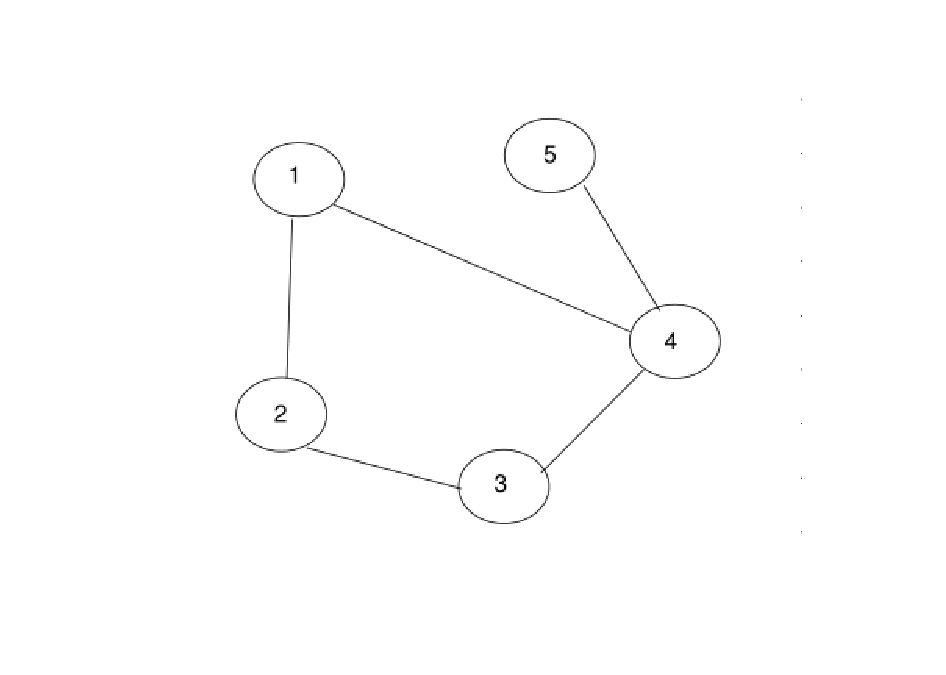
\includegraphics[width=1.8in]{delay/tuopu1.eps}}
            \subfigure[]{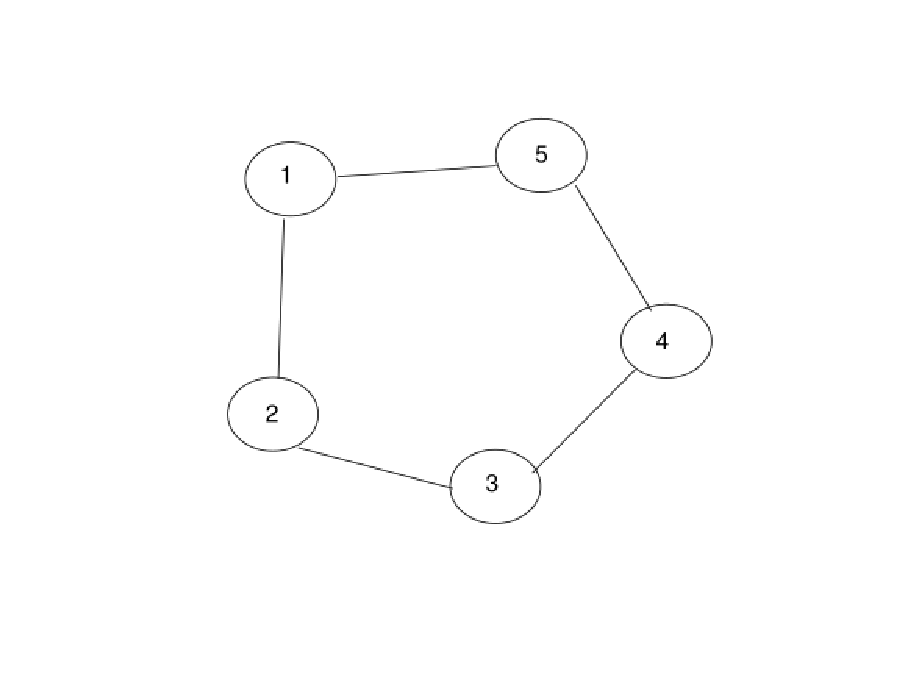
\includegraphics[width=1.8in]{delay/tuopu2.eps}}
            \subfigure[]{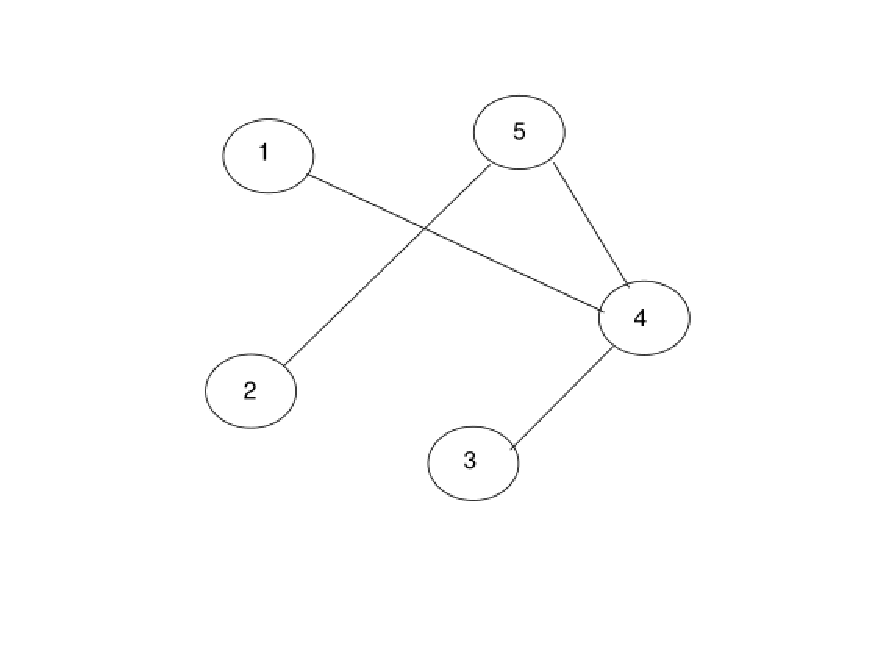
\includegraphics[width=1.8in]{delay/tuopu3.eps}}
     \end{center}
  \caption{网络系统在不同马氏链状态下可能的拓扑结构图.}\label{tuopu}
  \end{figure}
\begin{figure}[!htb]
\begin{minipage}[t]{0.48\linewidth}\centering
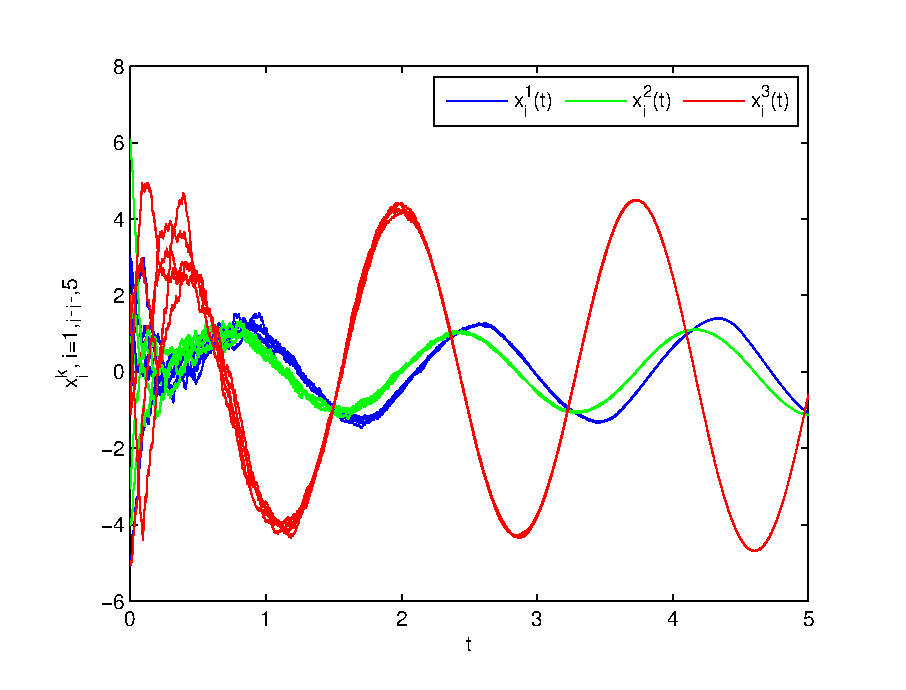
\includegraphics[width=3.2in]{noise/cestate.eps}\caption{在集中式激发采样策略下, 节点各个状态$x_i^j(t)$随时间演变图.}\label{cefig}
\end{minipage}~~
\begin{minipage}[t]{0.48\linewidth}\centering
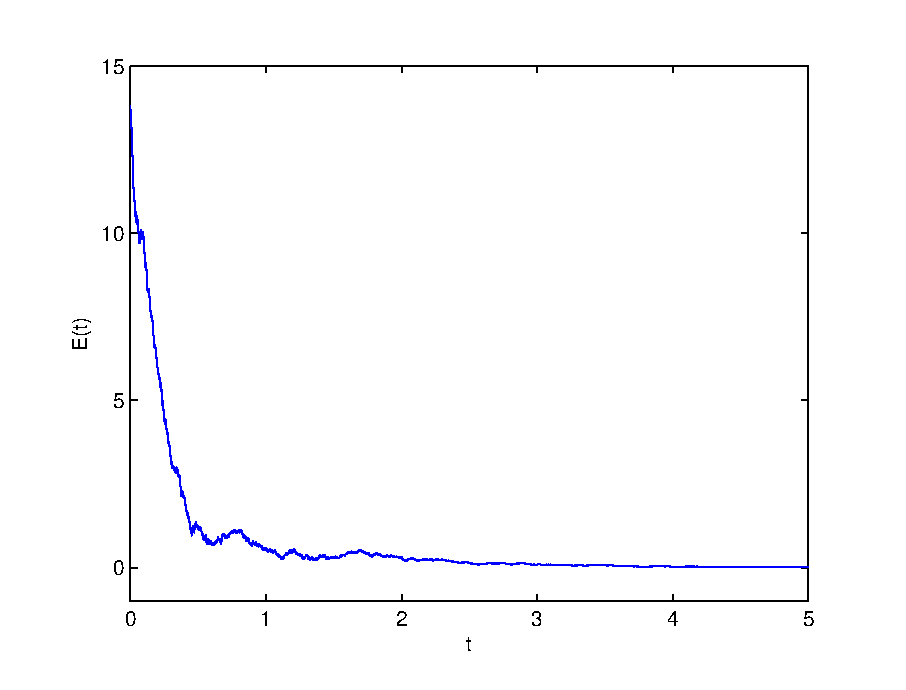
\includegraphics[width=3.2in,height=2.45in]{noise/ceEt.eps}\caption{在集中式激发采样策略下, 系统总误差$E(t)$随时间演变图.}\label{ceEt}
\end{minipage}
\end{figure}
\begin{figure}[!htb]
\begin{minipage}[t]{0.48\linewidth}\centering
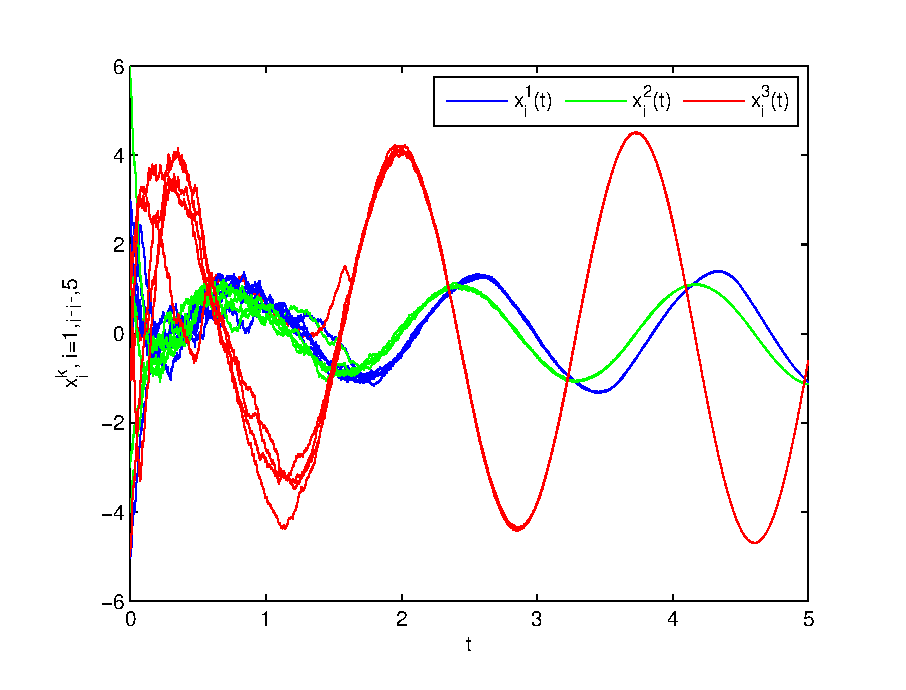
\includegraphics[width=3.2in]{noise/destate.eps}\caption{在分散式激发采样策略下, 节点各个状态$x_i^j(t)$随时间演变图.}\label{defig}
\end{minipage}~~
\begin{minipage}[t]{0.48\linewidth}\centering
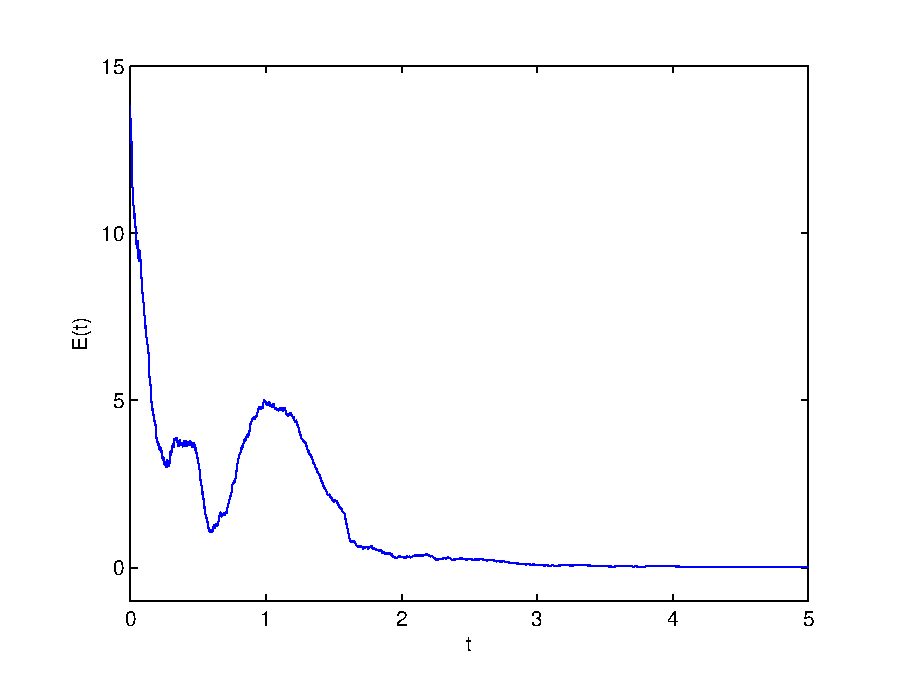
\includegraphics[width=3.2in,height=2.45in]{noise/deEt.eps}\caption{在分散式激发采样策略下, 系统总误差$E(t)$随时间演变图.}\label{deEt}
\end{minipage}
\end{figure}
马尔可夫链$\{r_t, t\geq0\}$是定义在有限状态空间$\{1,2,3\}$上, 其每个状态的平均逗留时间服从参数为$0.1$的指数分布, 并且转移率是部分未知的, 转移率矩阵如下:
        $$
          \left(
            \begin{array}{ccc}
              -8 & ? & ? \\
              5 & -8 & 3 \\
              ? & ? & -8 \\
            \end{array}
          \right).
          $$
    其中$"?"$表示未知转移率.

    复杂网络所有可能的拓扑结构如\autoref{tuopu}. 相应的控制节点集为$\mathcal{D}_1=\{2,4,5\}, \mathcal{D}_2=\{1,3,5\}$, 和$\mathcal{D}_3=\{1,2,3\}$是相应马尔可夫链状态下的牵制节点集.

    选取参数$\Gamma=I_3$, $\Delta=11.7I_3$. 为了估计 QUAD 条件中的参数$\xi$, 这里先求$f$的 Jacobin 矩阵如下:
        \begin{align*}
        J_1=\left(
              \begin{array}{ccc}
                3.0318 & 9.78 & 0 \\
                1 & -1 & 1 \\
                0 & -14.97 & 0 \\
              \end{array}
            \right),
        J_2=\left(
              \begin{array}{ccc}
                -2.445 & 9.78 & 0 \\
                1 & -1 & 1 \\
                0 & -14.97 & 0 \\
              \end{array}
            \right).
        \end{align*}
\begin{figure}[!htb]
\begin{minipage}[t]{0.48\linewidth}\centering
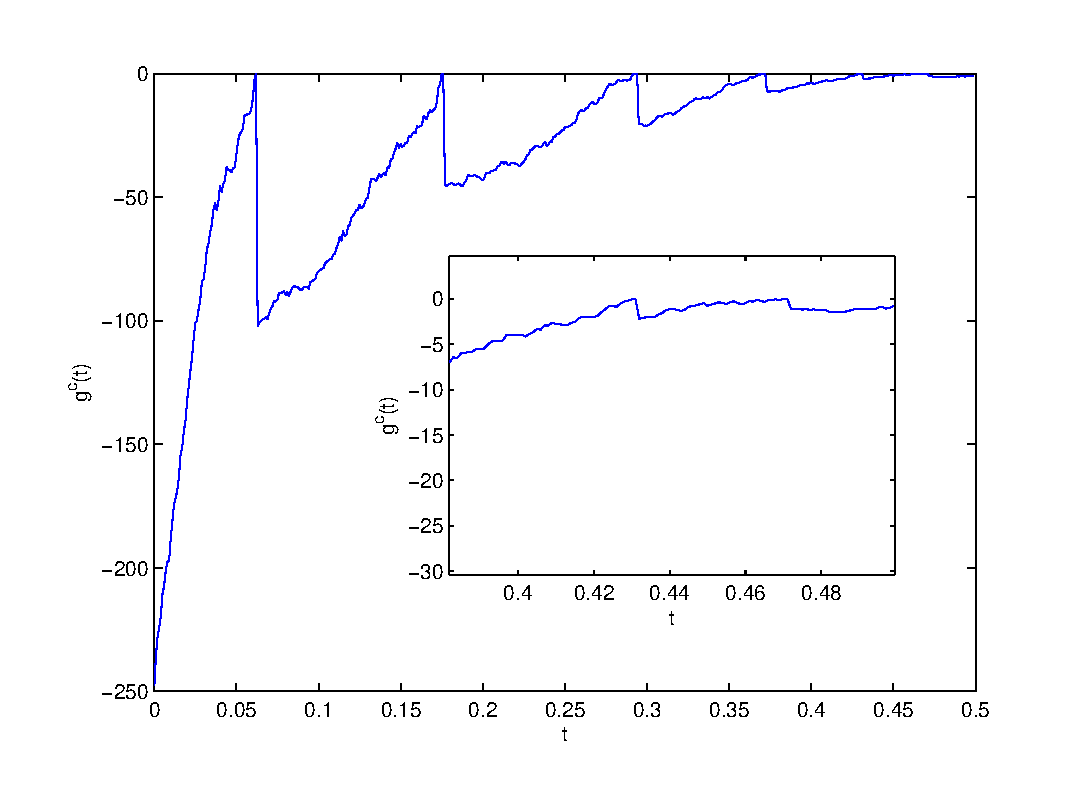
\includegraphics[width=3.2in]{noise/gct.eps}\caption{集中式激发函数 \eqref{trig-f} 变化图.}\label{gt}
\end{minipage}~~
\begin{minipage}[t]{0.48\linewidth}\centering
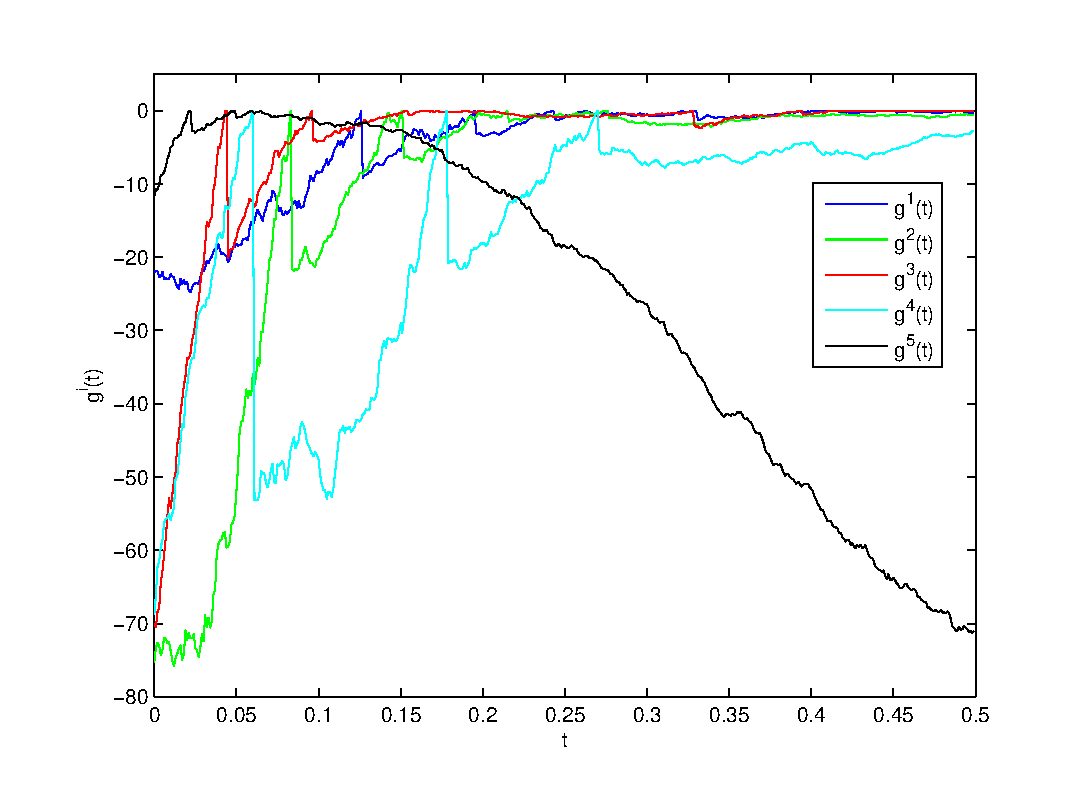
\includegraphics[width=3.2in]{noise/git.eps}\caption{分散式激发函数 \eqref{detrig-f} 变化图.}\label{degt}
\end{minipage}
\end{figure}

        通过计算可知, $f$所有的 Jacobin 矩阵的最大特征值为$9.1207$. 于是可得$\xi=\epsilon-9.1207$. 因为$\xi$是正数, 故可取$\epsilon=11.7$, 此时$\xi=11.7-9.1207=2.5793$.

    为了保证\autoref{thm:cen} 和\autoref{thm:decen} 的条件满足, 这里选取$c=25, \epsilon=15, \pi_1=\pi_2=\pi_3=8$, 以及$a_1=a_2=a_3=8.5$.节点的初值状态$x_1(0)=(3,1,-1)^\top$, $x_2(0)=(1,2,-5)^\top$, $x_3(0)=(-5,-4,-1)^\top$, $x_4(0)=(-1,6, 2)^\top$, $x_5(0)=(8,-3,1)^\top$, 以及$s(0)=(1,-1,2)^\top$.
    定义系统同步误差为
        $$E(t)=\sqrt{\sum_{i=1}^5\sum_{j=1}^3(x_i^j(t)-s^j(t))^2}.$$

    网络系统的微分方程求解方法利用的是欧拉迭代法, 步长为$0.001$, 迭代时间为$[0, 5]$, 数值解的结果以图片的形式给出, 见\autoref{cefig}$-$\autoref{tritimes}.

    从\autoref{cefig} 和\autoref{ceEt} 可以看出, 基于集中式事件激发采样策略 \eqref{trig-f} 下, 复杂网络系统的每一个节点每一维度的状态向量随着时间的演变慢慢地趋于同步状态, 并且系统同步误差从$10$迅速递减到$0$. 同样的, 在分散式事件激发采样策略下, \autoref{defig} 和\autoref{deEt} 展示了复杂网络系统各个节点的状态随着时间的演变趋于一致, 并且系统误差以较大的速度收敛于$0$.

    为了更好的展现事件激发的过程, \autoref{gt} 和\autoref{degt} 给分别出了在集中式事件激发采样策略和分散式事件激发采样策略下的激发函数的变量情况. 从图中可以看到, 集中式和分散式的激发函数值都是负数. 当激发函数是左极限等于零的时候, 此时事件被激发, 测量误差就等于零, 从而使得激发函数的值就等于同步误差的相反数, 此后, 测量误差有开始慢慢的增大至同步误差时, 事件就再一次被激发. 因此事件激发函数是具有周期缩短且函波峰逐渐平缓趋于零的性质. 集中式事件激发策略和分散式事件激发策略的不同点在于, 集中式激发策略只有一个激发函数, 其激发函数是根据系统所有节点的策略误差和同步误差的距离定义的, 而分散式事件策略要求每一个节点都有自己的激发函数, 其激发函数是根据节点自身的策略误差和同步误差的距离定义的.

\begin{figure}
\begin{center}
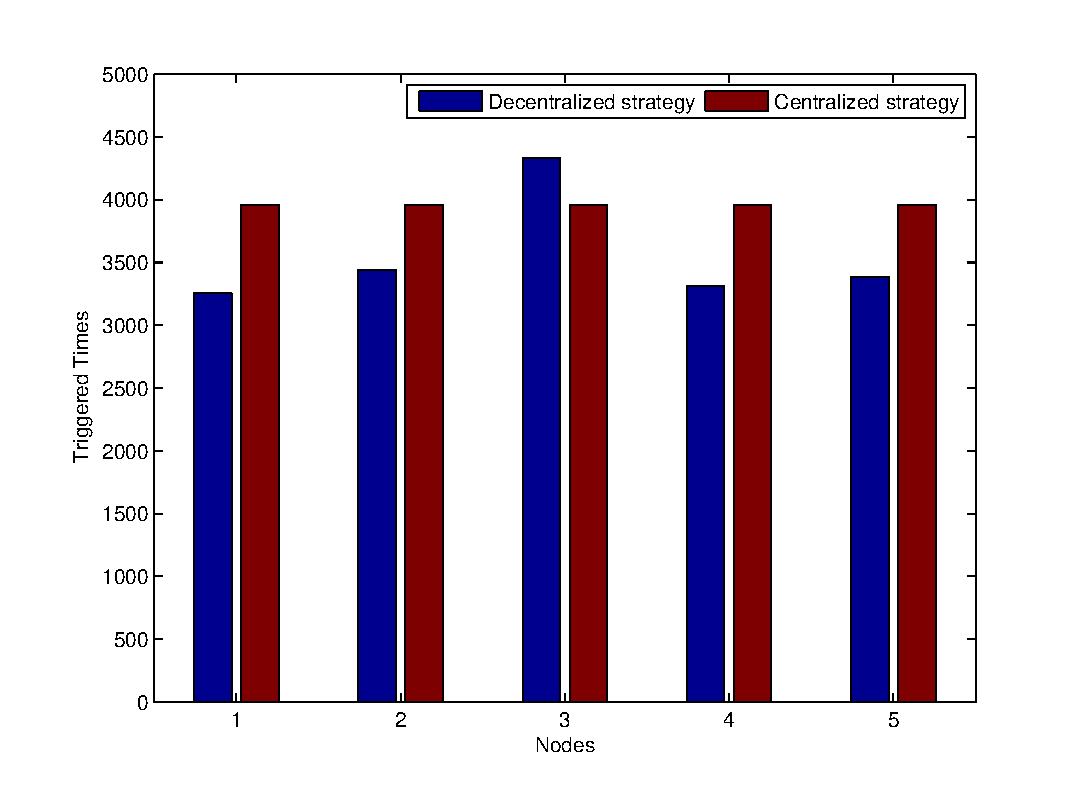
\includegraphics[width=3.2in]{noise/trigger.eps}\caption{在集中式激发采样策略和分散式激发采样策略下, 节点激发次数对比图.}\label{tritimes}
\end{center}
\end{figure}

    \autoref{tritimes} 给出了两种事件激发的激发次数, 从图中可以看出, 除了节点$3$外, 集中式的激发次数要高于分散式的激发次数. 从系统的平均激发次数来看, 集中式策略的激发次数也是高于分散式策略的激发次数. 这说明了分散式激发策略具有更低的更新频率和信息传输频率, 从而更节省能量, 但是分散式策略需要计算每个节点的激发函数, 因此也会导致较大的计算负荷.

\section{小结}
    本节主要讨论了带有部分未知转移率、随机噪声扰动、以及随机耦合强度的马氏切换复杂网络同步问题. 分别设置集中式和分散式的事件激发采样控制策略, 并在两种激发策略下分别给出了同步判据.
%    This paper researches the synchronous problem of Markovian switching complex networks with partly unknown transition rates, stochastic noise, and random coupling strength. By introducing new event-triggered functions, constructing a suitable stochastic Lyapunov-Krasovskii function, the sufficient synchronization criteria are derived respectively under both centralized and decentralized event-triggered control propotol. Simulation has shown that, by using the event-triggered strategy, the networks can achieve synchronization in relatively short time, and the decentralized event-triggered strategy have lower updating and transmission frequently compared with centralized event-triggered strategy.
